\documentclass[t,aspectratio=169,xcolor=dvipsnames]{beamer}

\usepackage{soul}
\usepackage{multicol}
\usepackage[utf8]{inputenc}
\usepackage{amsmath}
\usepackage{physics}
\usepackage{siunitx}
\usepackage{graphicx}
\usepackage{multirow}
\usepackage{mathtools}

% ----------------------------------------------------------------------------------------------------------------------------------------

\title{
\includegraphics[width=45pt]{oepecsetlogo.png}\\(KTXFI2EBNF) Physics II. Lecture}

\author{Dr.~Gábor FACSKÓ, PhD\\\tiny Assistant Professor / Senior Research Fellow\\\textit{facsko.gabor@uni-obuda.hu}}

\institute{\Tiny Óbuda University, Faculty of Electrical Engineering, 1084 Budapest, Tavaszmező u. 17.\\Wigner Research Centre for Physics, Department of Space Physics and Space Technology, 1121 Budapest, Konkoly-Thege Miklós út 29–33.\\ \url{https://wigner.hu/~facsko.gabor}}

\date{November~10,~2025}

\logo{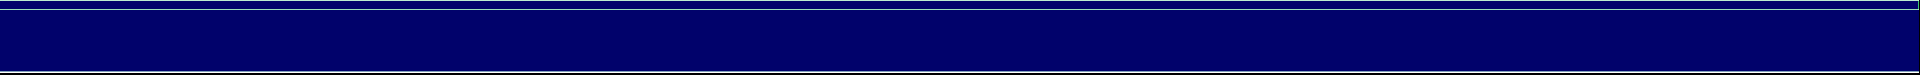
\includegraphics[height=0.9 true cm]{kekcsik.png}}

% ----------------------------------------------------------------------------------------------------------------------------------------

\begin{document}

\frame{\titlepage}

% ----------------------------------------------------------------------------------------------------------------------------------------

\begin{frame}%[fragile,squeeze,allowframebreaks]
\frametitle{Slides, Moodle, GitHub}
\begin{itemize}
\setlength{\parskip}{0pt}
\setlength{\itemsep}{0pt}
\item I had no time to translate the Hungarian text on the images into English. Sorry — it’s coming soon\dots
\end{itemize}
\end{frame}

% ----------------------------------------------------------------------------------------------------------------------------------------

\begin{frame}[fragile,squeeze,allowframebreaks]
\frametitle{Where are we?}
\begin{itemize}
\setlength{\parskip}{0pt}
\setlength{\itemsep}{0pt}
\item \st{Motion of charged particles in electromagnetic fields.}
  \item \st{Elements of quantum mechanics. Heisenberg's uncertainty principle. The stationary Schrödinger equation and its applications.}
\item \st{Limits of the classical conceptual framework. Thermal radiation. Photoelectric effect. Compton effect. The dual nature of electromagnetic radiation. The dual nature of particles.}
\item \st{Moving reference frames. Inertial forces in accelerating reference frames. Elements of special relativity. Dirac-equation, antimatter.}
\item \st{The classical theory of atomic structure (Rutherford, Franck-Hertz experiment, Bohr model, quantum numbers, Pauli exclusion principle).}
\item \st{Physics of condensed matter. Metallic bonding. Electrical conduction in metals based on the free electron model and the wave model. Hall effect. Band theory of solids.}
\pagebreak
\item \st{Semiconductors. Elements of Fermi-Dirac statistics.} \textbf{Thermoelectric phenomena. Magnetic properties.}
\item \textbf{Ferroelectricity. Piezoelectricity and electrostriction. Liquid crystals. Superconductivity.}
\item Luminescence. Lasers. Basic knowledge of nuclear physics. Basic knowledge of particle physics.
\end{itemize}
\end{frame}

% ----------------------------------------------------------------------------------------------------------------------------------------

\begin{frame}[fragile,squeeze,allowframebreaks]
  \frametitle{Contact and Contact Potential}
 \begin{center}
\includegraphics[width=0.57\textwidth]{images-20251110/erintkezesi_3_1.png}
\includegraphics[width=0.25\textwidth]{images-20251110/erintkezesi_3_2.png}\\ Alessandro Volta  (1745 – 1827)
\end{center}

\pagebreak
\begin{center}
\includegraphics[width=0.7\textwidth]{images-20251110/erintkezesi_4_1.png} \\ Alessando Volta (1745 – 1827)
\end{center}

\pagebreak
\begin{center}
\includegraphics[width=0.9\textwidth]{images-20251110/erintkezesi_5_1_english.png} \\ Volta's battery
\end{center}

\pagebreak
\begin{itemize}
  \setlength{\parskip}{0pt}
  \setlength{\itemsep}{0pt}
\item When two different metals are brought into contact, a contact (or Volta) potential $U_k$ arises between external points near the contact surfaces.\\
\begin{center}
\includegraphics[width=0.4\textwidth]{images-20251110/erintkezesi_6_1.png}
\end{center}

 \pagebreak
\item Volta potential: potential difference between external points near different metal surfaces (AB).
 \item Galvani potential: potential difference between internal points close to the interface inside the metals (A'B').\\  
\begin{center}
\includegraphics[width=0.35\textwidth]{images-20251110/erintkezesi_7_1.png}
\end{center}

\pagebreak
\item Contact potential originates from differing Fermi levels and work functions; electrons flow until an electric double layer with voltage $U_k=\phi_1-\phi_2$ stops further net transfer.\\
\begin{center}
\includegraphics[width=0.7\textwidth]{images-20251110/erintkezesi_8_1_english.png}
\end{center}
\item \underline{Detailed explanation based on the band theory of metals:} 
Before contact, the Fermi levels of different metals – which therefore have different work functions – do not coincide.  After contact, electrons move from metal 1, which has the higher Fermi level and the smaller work function, into metal 2. As negative electrons leave metal 1, an electron deficiency (an apparent positive excess) develops compared to its original neutral state; therefore, its potential becomes more positive, and its energy levels – including its Fermi level – shift downward.  Meanwhile, metal 2 receives electrons, creating an electron surplus; its potential becomes more negative, and its Fermi level shifts upward.

\pagebreak
\item Volta's Contact Potential Series
\begin{itemize}
  \setlength{\parskip}{0pt}
  \setlength{\itemsep}{0pt}
  \item Volta ordered metals according to contact potentials: Al -- Zn -- Pb -- Sn -- Sb -- Bi -- Fe -- Cu -- Ag -- Au -- Pt -- C.
  \item This ordering is known as Volta's contact potential series.
  \item These conductors are called Type I conductors. 

\pagebreak
\item If a third metal with contact potential $\Phi_{3}$  is inserted between a first metal with contact potential $\Phi_{1}$, and a second metal with contact potential $\Phi_{2}$, so that they are in mutual contact, then the contact potential difference between points A and B will be the same as if only metals 1 and 2 were present.
\begin{center}
\includegraphics[width=0.95\textwidth]{images-20251110/erintkezesi_10_1.png}
\end{center}
  
\pagebreak
\item In closed circuits of dissimilar conductors, contact potentials sum to zero; no net current flows solely from differing contact potentials.
\begin{center}
\includegraphics[width=0.4\textwidth]{images-20251110/erintkezesi_10_2.png}
\end{center}
\end{itemize}
\end{itemize}
\end{frame}

% ----------------------------------------------------------------------------------------------------------------------------------------

\begin{frame}[fragile,squeeze,allowframebreaks]
\frametitle{Thermoelectric Phenomena: Seebeck and Peltier Effects}
\begin{itemize}
  \setlength{\parskip}{0pt}
  \setlength{\itemsep}{0pt}
\item \underline{Seebeck effect}:  a closed circuit made of two different metals with junction temperatures $t_A$ and $t_B$ produces an electromotive force $U_t=\alpha (t_A-t_B)$ and a thermoelectric current $I_t=U_t/R$. $\alpha$ is the Seebeck coefficient (V/K).
\begin{columns}  
\begin{column}{0.3\textwidth}
\begin{center}
\includegraphics[width=0.9\textwidth]{images-20251110/erintkezesi_12_1.png}\\
\includegraphics[width=0.2\textwidth]{images-20251110/erintkezesi_12_2.png}
\end{center} 
\end{column}
\begin{column}{0.65\textwidth}
\begin{itemize}
\item If we create a temperature difference between the contact points A and B of a closed circuit composed of two different metals 1 and 2, the galvanometer inserted into the circuit indicates a current. That is, due to the temperature difference between the contact points A and B, an electric current flows in the circuit. The generated current is called the thermoelectric current, and the closed loop consisting of the two metals is called a thermocouple or thermal element. This phenomenon is the Seebeck effect.
\end{itemize}
\end{column}
\end{columns}

\pagebreak
\item Let, for example, $t_{A} > t_{B}$ and $W_{k1} < W_{k2}$.
\item In this case, electrons pass from metal 1, which has the smaller work function, into metal 2 at the surface belonging to point A.
\item Thus, the contact potential $U_{kA}$ of the electric double layer at location A becomes larger than the contact potential $U_{kB}$ at the colder point B.
\item Since the contact potentials corresponding to locations A and B have opposite “directions,” a so-called thermoelectric voltage  $$U_{t} = U_{kA} - U_{kB}$$   appears.

\pagebreak
\item This thermoelectric voltage sustains in the circuit with resistance $R$ the thermoelectric current of magnitude  $$ I_{t}=\frac{U_{t}}{R}=\frac{U_{kA}-U_{kB}}{R}.$$
\item Here  $$U_{t}=\alpha\left(t_{A}-t_{B}\right),$$ where $\left[\alpha\right]=\frac{V}{C^{\circ}}$ is the Seebeck coefficient, and $t_{A}$ and $t_{B}$ are the temperatures (in $C^{\circ}$) of the contact points.

  
\pagebreak
\item Applications: thermomagnet, thermobattery, thermocross (?)\\
\begin{center}
\includegraphics[width=0.2\textwidth]{images-20251110/erintkezesi_14_1.png}
\includegraphics[width=0.2\textwidth]{images-20251110/erintkezesi_14_2.png}
\includegraphics[width=0.2\textwidth]{images-20251110/erintkezesi_14_3_english.png}
\end{center}

\pagebreak
\item \underline{Peltier effect}: If two different metals are in contact and a direct current of magnitude $I$ flows through the contact or soldering point, then—besides the Joule heat—the contact or soldering point heats up or cools down depending on the direction of the current $I$.

\begin{columns}
\begin{column}{0.3\textwidth}    
 \begin{center}
\includegraphics[width=0.9\textwidth]{images-20251110/erintkezesi_15_1.png}
\end{center}
\end{column}
\begin{column}{0.7\textwidth}
\begin{itemize}
\item According to measurements, the \underline{Peltier heat} generated at the contact during time $\tau$ is  
$$ Q=\Pi I \tau, $$  
where $\Pi$ is the Peltier coefficient (V).
\item The thermoelectric coefficients are related by the Kelvin relation: $\Pi=\alpha t$, where $\alpha$ is the Seebeck coefficient and $t$ is the temperature in $C^{\circ}$.
\end{itemize}
\end{column}
\end{columns}

\pagebreak
\item The Peltier effect can be explained by the contact potential.
\item Let the conductor system consist of metals 1–2–1. Let the contact potentials of the metals be $\phi_{1}$, $\phi_{2}$, $\phi_{1}$, and let $\phi_{2} > \phi_{1}$.\\
\begin{center}
\includegraphics[width=0.65\textwidth]{images-20251110/erintkezesi_16_1_english.png}
\end{center}

\item In this case, in the electric field associated with the contact potential $U_{k}$ at the soldering point B, the electrons accelerate and their energy increases.

\pagebreak
\begin{center}
\includegraphics[width=0.6\textwidth]{images-20251110/erintkezesi_16_1_english.png}
\end{center}

\item The excess energy gained in this way manifests itself as heating at point B through collisions with the ions of the metal lattice.
\item In the opposite electric field corresponding to the contact potential $U_{k}$ at point A, however, the electrons slow down, their energy decreases, and therefore the contact at point A cools.
\item You can cool the chips of CCD cameras using the Peltier Effect!!!
\end{itemize}
\end{frame}

% ----------------------------------------------------------------------------------------------------------------------------------------

\begin{frame}[fragile,squeeze,allowframebreaks]
\frametitle{Magnetic Properties of Solids -- Dia-, Para-, and Ferromagnetism}
\begin{itemize}
\setlength{\parskip}{0pt}
\setlength{\itemsep}{0pt}
\item Magnetic Properties of Solids: According to the Bohr model, electrons move in well-defined circular orbits around the nucleus. Since an electron performs circular motion with a period $T$ (where $[T] = \mathrm{s}$), the moving charge generates a circular current. This current, in turn, produces a magnetic field around itself, according to the right-hand rule. The resulting magnetic field corresponds to that of a magnetic dipole.
\vskip -30 pt
\begin{columns}
\begin{column}{0.3\textwidth}
 \vskip 20 pt
\begin{center}
\includegraphics[width=0.9\textwidth]{images-20251110/magnesesseg_2_1.png}
\end{center}
\end{column}
\begin{column}{0.7\textwidth}
\begin{itemize}
\setlength{\parskip}{0pt}
\setlength{\itemsep}{0pt}
\item The strength of the circular current: $I = \frac{q_{electron}}{T}$, where $q_{electron}$ is the charge of the electron and $T$ is the electron's rotation period.
\item The magnitude of the magnetic dipole moment $m$ is: {\vskip -5 pt} $$m = I \cdot A = \frac{q_{electron}}{T} \cdot r^{2}\pi.$$ 
\item \underline{Magnetization:} The magnetic moment per unit volume is called the magnetization: {\vskip -15 pt} $$\mathbf{M} = \frac{\mathbf{m}}{V}.$$
\end{itemize}
\end{column}
\end{columns}

\pagebreak
\item The presence of matter (i.e., when not considered in vacuum) modifies the magnetic induction compared to its vacuum value.
\item In vacuum: $\mathbf{B} = \mu_{0} \mathbf{H}$. In matter: $\mathbf{B} = \mu_{0} \mu_{r} \mathbf{H}$.
\item In matter, the magnetic induction can also be written using the magnetization vector: $\mathbf{B} = \mu_{0}\mathbf{H} + \mathbf{M}$.
\item Therefore: {\vskip -30 pt}
\begin{eqnarray*}
  \mu_{0}\mu_{r}\mathbf{H} &=& \mu_{0}\mathbf{H} + \mathbf{M}\\
  \mu_{0}\mu_{r}\mathbf{H} &-& \mu_{0}\mathbf{H} = \mathbf{M}\\
 \mu_{0}\mathbf{H}(\mu_{r}-1) &=& \mathbf{M}. 
\end{eqnarray*}
\item \underline{Magnetic susceptibility:} The quantity $\kappa = \mu_{r} - 1$ is called the magnetic susceptibility.
\item Thus, the equation becomes: {\vskip -20 pt} $$\mu_{0}\mathbf{H}\kappa = \mathbf{M}.$$

\pagebreak
\item Introducing $\kappa$ is useful because it allows us to classify solid materials according to their magnetic properties.
\item Dia-, Para-, and Ferromagnetism
\begin{itemize}
\setlength{\parskip}{0pt}
\setlength{\itemsep}{0pt}
\item If $\kappa < 0$ and $\kappa \ll 1 \Rightarrow \mu_{r} \approx 1 \Rightarrow$ a small rod made of such a material aligns opposite to the magnetic field $\Rightarrow$ DIAMAGNETIC material.
\item If $\kappa > 0$ and $\kappa \ll 1 \Rightarrow \mu_{r} \approx 1 \Rightarrow$ a small rod made of such a material aligns with the magnetic field $\Rightarrow$ PARAMAGNETIC material.
\item If $\kappa \gg 1$ and depends on the magnetic field strength, and $\mu_{r}$ is on the order of $10^{3}$ $\Rightarrow$ such a material behaves similarly to a paramagnetic material $\Rightarrow$ FERROMAGNETIC material.
\end{itemize}

\pagebreak
\item Hysteresis (''memory curve'')
  \begin{columns}
    \begin{column}{0.2\textwidth}
 \begin{center}
\includegraphics[width=1.3\textwidth]{images-20251110/magnesesseg_5_1_modified.png}
\end{center}
\tiny{\textcolor{ForestGreen}{The area enclosed by the curve corresponds to the work required for magnetization. Small area $\Rightarrow$ soft magnet. Large area $\Rightarrow$ hard magnet.}}
\end{column}
\begin{column}{0.89\textwidth}
\vskip -20 pt
\begin{enumerate}
\setlength{\parskip}{0pt}
\setlength{\itemsep}{0pt}
\item Increasing the external field strength $\Rightarrow$ the magnetic induction initially increases rapidly, then reaches saturation: INITIAL (VIRGIN) CURVE.
\item When the external field is reduced to zero, magnetic induction still remains in the material: REMANENT INDUCTION.
\item By increasing the external field strength in the negative direction, the magnetic induction in the material can be reduced to zero.
\item \underline{Coercive force:} The value of the external field strength at which the magnetic induction in the material becomes zero is called the coercive field strength, or coercive force.
\item Increasing the external field further in the negative direction causes the magnetic induction to become negative and approach negative saturation.
\item Increasing the external field from a negative value toward positive values again, the magnetic induction becomes zero at a certain external field strength, then changes sign and eventually reaches positive saturation at higher field values.
\end{enumerate}
\end{column}
\end{columns}

\pagebreak
\item Materials with high coercive force and high remanence are suitable for use as permanent magnets.
\item As the temperature increases, a ferromagnetic material eventually becomes paramagnetic.
\item \underline{Curie point:} The lowest temperature at which a ferromagnetic material becomes paramagnetic is called the Curie point.
\item \underline{Magnetostriction:} A buzzing sound can often be heard near high-voltage transformers. This is due to magnetostriction. The essence of the phenomenon is that in a varying magnetic field, the dimensions of metal sheets (in transformers) or wires (in conductors) change. These dimensional changes produce pressure variations in the air, which propagate as longitudinal disturbances - perceived as sound.
\end{itemize}
\end{frame}

% ----------------------------------------------------------------------------------------------------------------------------------------

\begin{frame}[fragile,squeeze,allowframebreaks]
\frametitle{Ferroelectricity, Piezoelectricity, Electrostriction}
\begin{itemize}
\setlength{\parskip}{0pt}
\setlength{\itemsep}{0pt}
\item \underline{Ferroelectricity:} Certain insulating materials, i.e., dielectrics, behave in an electric field similarly to how iron behaves in an external magnetic field. This phenomenon is called ferroelectricity.
\item \underline{Ferroelectric crystal:} Dielectric materials that exhibit ferroelectric behavior when placed in an external electric field are called ferroelectric crystals.
\vskip -20 pt
  \begin{columns}
    \begin{column}{0.3\textwidth}
  \vskip 10 pt
  \begin{center}
\includegraphics[width=0.9\textwidth]{images-20251110/magnesesseg_8_1.png}
\end{center}
\end{column}
\begin{column}{0.7\textwidth}
\begin{itemize}
\setlength{\parskip}{0pt}
\setlength{\itemsep}{0pt}
\item In such materials, the electric displacement vector $D$ exhibits a hysteresis (memory) effect similar to that observed in ferromagnetic materials.
\item The electric displacement vector is given by: $$\mathbf{D} = \epsilon_{0}\epsilon_{r}\mathbf{E}.$$ Here, the relative permittivity $\epsilon_{r}$ is not constant but varies with the external electric field, and it may reach values on the order of $10^{4}$.
\end{itemize}
\end{column}
\end{columns}

\pagebreak
\item \underline{Piezoelectricity}: mechanical deformation induces electric polarization (Curie brothers, 1880). When a crystal is deformed, oppositely charged polarization surfaces appear on opposite faces of the crystal. When the direction of the deforming force is reversed, the sign of the charges on the faces also reverses.
\item Forms: (1) dipoles are created during deformation; (2) existing dipoles are rearranged during deformation.
  \begin{center}
\includegraphics[width=0.36\textwidth]{images-20251110/magnesesseg_9_1_english.png}
\includegraphics[width=0.425\textwidth]{images-20251110/magnesesseg_9_2_modified.png}
\end{center}
\item Applications: lighters, gas igniters, \dots

\pagebreak
\item \underline{Electrostriction}: The phenomenon in which a crystal, when placed in an electric field, becomes deformed, stretched, or compressed is called electrostriction (Pierre Curie, 1881).
\item Electrostriction is the inverse of piezoelectricity.
\item In an alternating electric field, such crystals undergo oscillatory motion corresponding to the alternating voltage.
\item Applications: quartz clocks, diesel injectors, \dots
\end{itemize}
\end{frame}

% ----------------------------------------------------------------------------------------------------------------------------------------

\begin{frame}[fragile,squeeze,allowframebreaks]
\frametitle{Liquid Crystals}
\vskip -10 pt  
\begin{itemize}
\setlength{\parskip}{0pt}
\setlength{\itemsep}{0pt}
\item Friedrich Reinitzer (1857–1927), Austrian botanist — experiment with cholesteryl benzoate in 1888.
\begin{itemize}
\setlength{\parskip}{0pt}
\setlength{\itemsep}{0pt}
\item CRYSTAL $\xRightarrow[\text{heated to }145\,^{\circ}\text{C}]{\text{heating}}$ CLOUDY, OPAQUE LIQUID $\xRightarrow[\text{heated to }179\,^{\circ}\text{C}]{\text{heating}}$ CLEAR, TRANSPARENT LIQUID
\item A material with two melting points
\end{itemize}
\item Lehmann
\begin{itemize}
\setlength{\parskip}{0pt}
\setlength{\itemsep}{0pt}
\item Cloudy, opaque phase: optically anisotropic regions
\item New name: liquid–crystalline state
\end{itemize}
\item George H. Heilmeier, 1968: liquid crystals as materials suitable for microelectronics.
\item States of matter: SOLID $\Rightarrow$ LIQUID $\Rightarrow$ GAS $\Rightarrow$ PLASMA \textcolor{red}{$\leftarrow$LIQUID CRYSTAL}$\rightarrow$ the 5th state of matter (e.g., aqueous solutions of soaps and detergents, silk fibers, vessel walls, cell membranes). Macroscopically liquid, microscopically solid-like.

\pagebreak

\item Types of liquid crystals:
\begin{itemize}
\item The ordering of the centers of mass is preserved, but orientational disorder is present.
\item The ordering of the centers of mass disappears, but orientational order remains.
\end{itemize}

\item \underline{Liquid crystal:} Liquid crystals are materials in which the complete, simultaneous ordering of the molecular centers of mass and the molecular axes does not occur.

\item Groups of liquid crystals:
\begin{itemize}
\item Thermotropic: formed from the crystalline state upon heating.
\item Lyotropic: formed from the crystalline state in the presence of a solvent.
\end{itemize}

\pagebreak
\item Classification of liquid crystals according to G. Friedel (1865–1933):
\begin{itemize}
\item SMECTIC
\begin{columns}
\begin{column}{0.5\textwidth}
\begin{center}
\includegraphics[width=0.45\textwidth]{images-20251110/magnesesseg_14_1.png}
\includegraphics[width=0.45\textwidth]{images-20251110/magnesesseg_14_2.png}
\end{center}
\end{column}
\begin{column}{0.5\textwidth}
\begin{itemize}
  \item Layered structure
  \item Molecules in the layers are oriented randomly.
  \item Layers can slide over each other.
  \item Thermotropic
\end{itemize}
\end{column}
\end{columns}

\pagebreak
\item NEMATIC
\begin{columns}
\begin{column}{0.5\textwidth}
\begin{center}
\includegraphics[width=0.49\textwidth]{images-20251110/magnesesseg_15_1.png}
\includegraphics[width=0.49\textwidth]{images-20251110/magnesesseg_15_2.png}
\end{center}
\end{column}
\begin{column}{0.5\textwidth}
\begin{itemize}
\item Molecules form thread-like chains.
\item Their axes are parallel, but they do not form layers.
\item Toothpick model.
\end{itemize}
\end{column}
\end{columns}

\pagebreak
\item CHOLESTERIC
\begin{columns}
\begin{column}{0.5\textwidth}
\begin{center}
\includegraphics[width=0.49\textwidth]{images-20251110/magnesesseg_16_1.png}
\includegraphics[width=0.49\textwidth]{images-20251110/magnesesseg_16_2.png}
\end{center}
\end{column}
\begin{column}{0.5\textwidth}
\begin{itemize}
\item Layered structure
\item In each layer, molecular axes are parallel.
\item In different layers, the molecular axes point in different directions (periodic rotation).
\item They rotate the polarization of light.
\end{itemize}
\end{column}
\end{columns}
\end{itemize}

\pagebreak
\item Types of Liquid-crystal display (LCD) displays:
\begin{itemize}
\item LCDs based on dynamic scattering:
\begin{itemize}
\item 1968: dynamic scattering — light is scattered by rotating, moving molecules.
\item Without applied voltage: transparent; with voltage: dark.
\item Electric current $\Rightarrow$ swirling ions $\Rightarrow$ light-scattering centers (dynamic scattering) $\Rightarrow$ ionic conduction, scattering on ions (dynamic scattering).
\end{itemize}
\hskip -30 pt
\begin{center}
\vskip -5 pt
\includegraphics[width=0.35\textwidth]{images-20251110/magnesesseg_17_1_english.png}
\includegraphics[width=0.35\textwidth]{images-20251110/magnesesseg_17_2_english.png}
\end{center}{\vskip -5 pt}
Transmission (transmissive) displays \hfill Reflection (reflective) displays

\pagebreak
\item Spatially controlled LCDs, i.e., the electrically controlled twisted–nematic cell:
\begin{itemize}
\item The twisted–nematic cell \textcolor{blue}{$\downarrow$} rotates the light polarization plane by $90^{\circ}$.
\begin{center}
\includegraphics[width=0.8\textwidth]{images-20251110/magnesesseg_18_1_english.png}
\end{center}
\end{itemize}

\end{itemize}
\end{itemize}
\end{frame}

% ----------------------------------------------------------------------------------------------------------------------------------------

\begin{frame}[fragile,squeeze,allowframebreaks]
  \frametitle{Superconductivity}
\begin{itemize}
  \setlength{\parskip}{0pt}
  \setlength{\itemsep}{0pt}

\item Experiments of Kamerlingh-Onnes (1853–1926), Dutch physicist:
\begin{itemize}
\item He succeeded in producing liquid helium (1908–1911).
\item He investigated the physical properties of metals at low temperatures, particularly electrical conductivity.
\item Measurement results: \hfill Measurement results with highly pure metal (Hg):
\end{itemize}

\begin{center}
  \includegraphics[width=0.9\textwidth]{images-20251110/klasszikus_kiserletek.png}
\end{center}
{\vskip -10 pt}
{\tiny\textcolor{ForestGreen}{The residual resistance observed at zero kelvin originates}\\{\vskip -8 pt}\textcolor{ForestGreen}{from impurities and structural defects within the metal.}}

\pagebreak
\item The electrical resistance of mercury and several other metals suddenly drops to zero a few degrees above absolute zero.\\
$T_{c}$ values: Hg: 4.17 K, Al: 1.14 K, Sn: 3.69 K
\item \underline{Critical temperature ($T_{c}$):}  
The temperature at which the electrical resistance of a material abruptly falls to zero is called the critical temperature.
\item \underline{Superconducting material:}  
Materials whose electrical resistance becomes zero below the critical temperature $T_{c}$ are referred to as superconductors.
\item \underline{First-type or Type I superconductors:}  
Pure metallic superconductors are classified as first-type (Type I) superconductors.
\item Copper, silver, and gold cannot be brought into a superconducting state.
\begin{itemize}
\item An electric current induced in a superconducting ring can persist for thousands of years, provided the material remains in the superconducting state.
\item Because $R = 0$, the current can flow indefinitely without resistive losses.
\end{itemize}

\pagebreak
\item Consequences and Properties:
\item \textbf{Magnetic threshold (critical field) curve:} \hfill \textbf{Critical current density curve:}\\
Example for mercury: \hfill Example for mercury:
\begin{center}
\includegraphics[width=0.375\textwidth]{images-20251110/szupravezetes_5_1_english.png}
\includegraphics[width=0.375\textwidth]{images-20251110/szupravezetes_5_2_english.png}
\end{center}

\pagebreak
\item In the three-dimensional $H$–$T$–$J$ space:
\begin{center}
\includegraphics[width=0.45\textwidth]{images-20251110/szupravezetes_6_1_english.png}\hfill
\includegraphics[width=0.45\textwidth]{images-20251110/szupravezetes_6_2_english.png}
\end{center}

\pagebreak
\item \underline{Second-type (Type II) superconductors:}  
Alloys, metallic compounds, and ceramic materials that exhibit superconductivity are called second-type superconductors. In their normal state, they are typically poor conductors with relatively high resistivity.
\item H–T characteristic curve of second-type superconductors:
\begin{center}
\includegraphics[width=0.3\textwidth]{images-20251110/szupravezetes_7_1_english.png}
\includegraphics[width=0.3\textwidth]{images-20251110/szupravezetes_7_2_english.png}
\end{center}

\pagebreak
\item \underline{High-Temperature Superconductivity (HTSC):}  
In 1986, Bednorz and Müller discovered that certain copper-oxide ceramics exhibit superconductivity above the boiling point of liquid nitrogen ($77\,K$), initiating the field of high-temperature superconductivity.
\item Materials that become superconducting above $77\,K$ (i.e., above the liquefaction temperature of nitrogen) are called high-temperature superconductors, or HTSC materials.
\begin{center}
\includegraphics[width=0.55\textwidth]{images-20251110/szupravezetes_8_1.png}
\end{center}

\pagebreak
\item \underline{Meissner–Ochsenfeld Effect:}  
When a material transitions into the superconducting state, it expels magnetic flux from within its interior — a phenomenon known as perfect diamagnetism or the Meissner effect.
\begin{center}
\begin{tabular*}{1.0\linewidth}[c]{ccc}
\includegraphics[width=0.2\textwidth]{images-20251110/szupravezetes_9_1.png} & \multirow{2}{*}{\includegraphics[width=0.25\textwidth]{images-20251110/szupravezetes_9_3.png}} & \multirow{2}{*}{\includegraphics[width=0.25\textwidth]{images-20251110/szupravezetes_9_2.png}} \\
\includegraphics[width=0.2\textwidth]{images-20251110/szupravezetes_9_4.png} &  \\
\end{tabular*}
\end{center}

\pagebreak
\item \underline{Bardeen–Cooper–Schrieffer (BCS) Theory:}  
John Bardeen (1908–1991), Leon N. Cooper (1930–), and John R. Schrieffer (1931–) formulated the microscopic explanation of superconductivity in 1957, for which they were awarded the Nobel Prize in 1972.
\item They established that $T_{c} \cdot M = \mathrm{const}$, where $M$ is the atomic mass.  
$\Rightarrow$ This indicates that the mass influences the vibrational states of atoms.  
$\Rightarrow$ In the superconducting state, electrons interact with lattice vibrations (phonons).
\item Electrons in the superconducting state form bound pairs.  
In the phonon field, electrons with opposite spins experience an effective attraction rather than repulsion, forming \textbf{Cooper pairs}.
\item The motion of other electrons in the lattice exerts a perturbing effect that counteracts pair formation.

\pagebreak
\item Cooper pairs are not permanent entities: they may break and recombine continually.
\item Electron pairs behave as particles with zero spin.  
$\Rightarrow$ The Pauli exclusion principle does not apply to them.  
Such particles obey \textbf{Bose–Einstein statistics} rather than Fermi–Dirac statistics.
\item When an electric field is applied, Cooper pairs accelerate collectively.
\item Energy is required to form Cooper pairs. This binding energy lowers the Fermi energy of the material, and a forbidden energy gap opens above the Fermi level in the band structure.

\pagebreak
\item \underline{Josephson Effect:}  
Brian David Josephson (1940–), as a young university student, published a seminal four-page paper in 1962 describing this phenomenon.
\item Cooper pairs can tunnel from one superconducting material to another through a thin insulating barrier placed between them.
\item The transfer mechanism is quantum tunneling:
\medskip
\begin{center}
\includegraphics[width=0.55\textwidth]{images-20251110/szupravezetes_12_1_english.png}
\includegraphics[width=0.35\textwidth]{images-20251110/szupravezetes_12_2_english.png}
\end{center}
\end{itemize}
\end{frame}

% ----------------------------------------------------------------------------------------------------------------------------------------

\begin{frame}
%\frametitle{Minden jó, ha a vége jó}

\vfill
\begin{center}
\textbf{\huge The End}

\bigskip
Thank you for your attention!
\end{center}
\vfill
\end{frame}

\end{document}
